\documentclass{vilniustech}
\vilniustechsetup{
    university={Vilniaus Gedimino technikos universitetas},
    faculty={Fundamentinių mokslų fakultetas},
    cathedral={Matematinės statistikos katedra},
    workTitle={Mokslinių tyrimų ir inovacijų pagrindų},
    workType={Namų darbas nr.1},
    workAuthorGroup={ITSfm-22},
    workAuthorName={Aurimas Šakalys},
    workRecipient={doc. dr. Rūta Simanavičienė}
}
\addbibresource{hw1.bib}
\VTDocumentBegin

\section{System security assurance: A systematic literature review}

\subsection{Straipsnio bibliografinis aprašas}
\VTTable{[
    caption = {Straipsnio bibliografinis aprašas},
    label = {biblio1:short}
    ]{
    colspec = {X[2] X[5]},
    column{1} = {font=\bfseries}
    }
    Autorius (-iai) & Ankur Shukla, Basel Katt, Livinus Obiora Nweke, Prosper Kandabongee Yeng, Goitom Kahsay Weldehawaryat \\
    Pavadinimas & System security assurance: A systematic literature review \\
    Publikavimo metai & 2022 \\
    Žurnalo pavadinimas, vol. & Computer Science Review, 45 \\
    Nuoroda į šaltinį & \url{https://doi.org/10.1016/j.cosrev.2022.100496} \\
}

\subsection{Kokia mokslinė problema sprendžiama analizuojamame darbe?}
Straipsnyje \parencite{SHUKLA2022100496} analizuojama sistemų saugos užtikrinimo metodika. Į analizę įtraukiami dėl informacijos ir komunikacijų technologijų (ICT) atsiradę įšukiai, kadangi įprastai naudojami sprendimai gali neapimti naujai kylančių problemų. Bendrieji kriterijai (CC) naudojami vertinant sistemų saugą yra riboti ir nepaslankūs.

\subsection{Darbo tikslas, keliamas analizuojamame darbe}
Atlikti sistemingą egzistuojančių reikalavimų, procesų ir veiklų analizę sistemų saugos užtikrinimui ir įvardinti esamus trūkumus.

\subsection{Uždaviniai, formuluojami analizuojamame darbe}
Kadangi straipsnyje \parencite{SHUKLA2022100496} atliekama sisteminė analizė, uždaviniai formuluojami tyrimo klausimais.

\VTTable{[
    caption = {Straipsnio keliami klausimai},
    label = {tasks1:short}
    ]{
    colspec = {X[1] X[18]},
    row{1} = {font=\bfseries}
    }
    Nr. & Klausimas \\
    1 & Kokios yra dabartinės tendencijos, sistemų saugos užtikrinimo srityje, apžvelgiant į procesus, metodus, gaires, įrankius,
    metrikas, įvertinimus/technikas, automatizavimą, standartus, ir
    taikomųjų programų dalykines sritis?\\
    2 & Su kokiais iššūkiais, apribojimais ir spragomis susiduriama sistemų saugos užtikrinimo srityje?\\
    3 & Kokios ateities tendencijos sistemų saugos užtikrinimo srityje? \\
    4 & Kaip galėtume klasivikuoti tiriamąją veiklą sistemų saugos užtikrinimo srityje?  \\
}

\subsection{Koks yra mokslinio darbo naujumas?}
Analizuojamos įvairios metodologijos, kriterijai, užtikrinimo lygiai, trūkumai, sistemos ir aplinkos. Visa ši analizė yra apibendrinama ir pateikiamas bendras rezultatas, kuris nereikalauja ateityje atlikti tokios pačios analizės, norint naudotis gautais rezultatais.  

\subsection{Koks literatūros apžvalgos tipas taikomas?}
Straipsnyje yra taikoma sisteminė literatūros apžvalga, kuria siekiama apibendrinti ir susintetinti daugelį empirinių tyrimų į vieną visumą. Tai labai tinkamas apžvalgos tipas, kadangi darbo tikslas - apibendrinti ir susistemizuoti egzistuojančius tyrimus.

\subsection{Koks empirinio tyrimo metodas taikomas?}
Miršrus, matavimų ir atvejo analizės metodas - nors darbe vykdomas apibendrinimas, yra vertinami ir matuojami į apibendrinimą įtraukiamų straipsnių kokybiniai rodikliai, vykdoma straipsnių atranka ir iš atranką perėjųsių straipsnių išrenkami reikiami duomenys.

\subsection{Kokie statistiniai metodai taikomi duomenų analizei?}
Miršrus, aprašomosios statistikos ir klasfikacijos analizė, atliekama vertinant ir atrenkant straipsnius.

\subsection{Kurį Bloom'o taksonomijos lygmenį atitinka šis mokslinis darbas ir kodėl?}

\subsection{Koks citavimo stilius naudojamas šiame darbe?}
Cituojama IEEE citavimo stiliumi.

\subsection{Kokioms mokslinių publikacijų citavimo duomenų bazėms priklauso žurnalas, kuriame publikuojamas šis straipsnis?}
\VTTable{[
    caption = {Straipsnio mokslometriniai rodikliai ir duomenų bazės},
    label = {scimetrics1:short}
    ]{
    colspec = {X[5] X[2] X[2]},
    row{1} = {font=\bfseries}
    }
    Duomenų bazės & CiteScore & Impact Factor \\
    \begin{enumerate}
    \item Zentralblatt MATH
    \item Scopus
    \item Science Citation Index Expanded
    \item INSPEC
    \end{enumerate} & 14.3 & 8.757 \\
}

\section{Standardizing information security - a structurational analysis}

\subsection{Straipsnio bibliografinis aprašas}
\VTTable{[
    caption = {Straipsnio bibliografinis aprašas},
    label = {biblio2:short}
    ]{
    colspec = {X[2] X[5]},
    column{1} = {font=\bfseries}
    }
    Autorius (-iai) & Annika Andersson, Karin Hedström, Fredrik Karlsson \\
    Pavadinimas & Standardizing information security - a structurational analysis \\
    Publikavimo metai & 2022 \\
    Žurnalo pavadinimas, vol., iss. & Information \& Management, 59, 3 \\
    Nuoroda į šaltinį & \url{https://doi.org/10.1016/j.ins.2022.07.053} \\
}

\subsection{Kokia mokslinė problema sprendžiama analizuojamame darbe?}
Straipsnyje \parencite{ANDERSSON2022103623} analizuojama kokią įtaką įvesčiai ir pralaidumo teisėtumui turi struktūros naudojamos de jure standartų vystyme.

\subsection{Darbo tikslas, keliamas analizuojamame darbe}
Bandoma atsakyti į klausimą, kokią įtaką įvesčiai ir pralaidumo teisėtumui turi struktūros naudojamos de jure standartų vystyme?

\subsection{Uždaviniai, formuluojami analizuojamame darbe}
Specifiniai uždaviniai straipsnyje nėra minimi, tačiau dalį jų galima suformuluoti.
Vienas uždavinys - išanalizuoti per 34 mėnesius dalyvaujant saugumo standartų vystymo procesuose surinktus duomenis.
?????

\subsection{Koks yra mokslinio darbo naujumas?}
Atlikus analizę buvo rastos dvi struktūros kurios labai skirtingai paveikė įvesties ir pralaidumo teisėtumą - konsensuso ir karybos struktūros. Buvo pastebėta, jog konsensuso sturktūra sustiprino įvesties ir pralaidumo teisėtumą, 

\subsection{Koks literatūros apžvalgos tipas taikomas?}
Naudojama atpasakojamoji apžvalga, siekiama literatūros pagalba pagrįsti tyrimo reikmę ir kryptį.

\subsection{Koks empirinio tyrimo metodas taikomas?}
Mišrus, naudojamas etnografinis ir laiko tyrimas, kadangi tyrėjai tiesiogiai dalyvauja standartų vystymo procesuose ir jų metu renka ir sistematizuoja surintus duomenis.

\subsection{Kokie statistiniai metodai taikomi duomenų analizei?}
Naudojama aprašomoji statistika ir klasifikavimas. 

\subsection{Kurį Bloom'o taksonomijos lygmenį atitinka šis mokslinis darbas ir kodėl?}

\subsection{Koks citavimo stilius naudojamas šiame darbe?}
Cituojama IEEE citavimo stiliumi.

\subsection{Kokioms mokslinių publikacijų citavimo duomenų bazėms priklauso žurnalas, kuriame publikuojamas šis straipsnis?}
\VTTable{[
    caption = {Straipsnio mokslometriniai rodikliai ir duomenų bazės},
    label = {scimetrics2:short}
    ]{
    colspec = {X[5] X[2] X[2]},
    row{1} = {font=\bfseries}
    }
    Duomenų bazės & CiteScore & Impact Factor \\
    
    \begin{enumerate}
    \item Data Manager
    \item ANBAR
    \item EDP Performance Review
    \item DP Directory
    \item ACM Computing Reviews
    \item Computer Abstracts
    \item Computer \& Control Abstracts
    \item Data Processing Digest
    \item Information Retrieval and Library Automation
    \item Information Science Abstracts
    \item Current Contents
    \item Quarterly Bibliography of Computers and Data Processing
    \item Engineering Index
    \item INSPEC
    \item Embase
    \item UMI Data Courier
    \item Mathematical Management & Physics Abstracts
    \item Management Contents
    \item Statistical Reference Index
    \item Cambridge Scientific Abstracts
    \item Academic Journal Guide (Chartered Association of Business Schools)
    \item Science Citation Index
    \item Social Sciences Citation Index 
    \end{enumerate}  & 13.1 & 10.328 \\
}

\section{Literatūra}

\section{Citavimo pavyzdžiai}

\subsection{Įvairių objektų citavimas}

Tinklalapio citavimas \parencite{webcitation}.
\begin{verbatim}
    \parencite{webcitation}
\end{verbatim}

Straipsnio citavimas \parencite{articlecitation}.
\begin{verbatim}
    \parencite{articlecitation}
\end{verbatim}

Knygos citavimas \parencite{bookcitation}.
\begin{verbatim}
    \parencite{bookcitation}
\end{verbatim}


\subsection{Citavimo komandos}

Parastas citavimas \cite{articlecitation}.
\begin{verbatim}
    \cite{articlecitation}
\end{verbatim}

Citavimas skliausteliuose \parencite{articlecitation}.
\begin{verbatim}
    \parencite{articlecitation}
\end{verbatim}

Citavimas poraštėje \footcite{articlecitation}.
\begin{verbatim}
    \footcite{articlecitation}
\end{verbatim}

Citavimas tekstu \textcite{articlecitation}.
\begin{verbatim}
    \textcite{articlecitation}
\end{verbatim}

\newpage
\section{Iliustracijų/lentelių pavyzdžiai}

\begin{figure}[H]
\begin{center}
    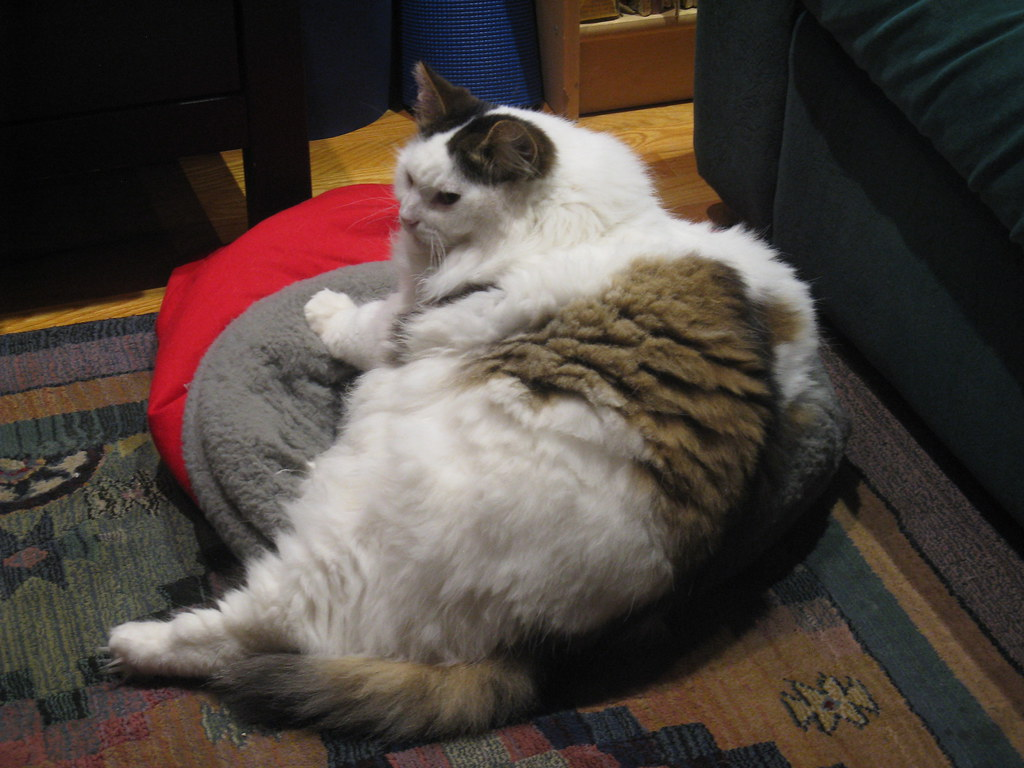
\includegraphics[height=6cm]{img/chonker.jpg}
    \caption{Gabalainis}
    \label{fig:fig1}
\end{center}
\end{figure}

\VTTable{[
    caption = {Trumpa lentelė},
    label = {table:short}
    ]{
    colspec = {XX},
    row{1} = {font=\bfseries}
    }
    Antraštė 1 & Antraštė 2 \\
    Lorem ipsum & Lorem ipsum \\
    Lorem ipsum & Lorem ipsum \\
}

\subsection{Nuorodos}

Nuoroda į iliustraciją \ref{fig:fig1} esančią \pageref{fig:fig1} puslapyje.
\begin{verbatim}
    \ref{fig:fig1} \pageref{fig:fig1}
\end{verbatim}

Nuoroda į trumpą lentelę \ref{table:short} esančią \pageref{table:short} puslapyje.
\begin{verbatim}
    \ref{table:short} \pageref{table:short}
\end{verbatim}

Nuoroda į ilgą lentelę \ref{table:long} esančią \pageref{table:long} puslapyje.
\begin{verbatim}
    \ref{table:long} \pageref{table:long}
\end{verbatim}

\VTTable{[
    caption = {Kelių puslapių lentelė},
    label = {table:long}
    ]{
    colspec = {XXX},
    rowhead = 1,
    row{1} = {font=\bfseries}
    }
    Antraštė 1 & Antraštė 2 & Antraštė 3 \\
    Lorem ipsum & Lorem ipsum & Lorem ipsum \\
    Lorem ipsum & Lorem ipsum & Lorem ipsum \\
    Lorem ipsum & Lorem ipsum & Lorem ipsum \\
    Lorem ipsum & Lorem ipsum & Lorem ipsum \\
    Lorem ipsum & Lorem ipsum & Lorem ipsum \\
    Lorem ipsum & Lorem ipsum & Lorem ipsum \\
    Lorem ipsum & Lorem ipsum & Lorem ipsum \\
    Lorem ipsum & Lorem ipsum & Lorem ipsum \\
    Lorem ipsum & Lorem ipsum & Lorem ipsum \\
}

\VTDocumentEnd